% =====================================================================
% Course documentation on the full official ACL template (acl_latex.tex,
% acl-org/acl-style-files, also used by NAACL), option `final`.
% Method: release/ (anonymous repo). Numbers: release/fuse.py, saved in
%   output/doc_fuse_ro11.*    11 languages, main result
%   output/doc_fuse_mlsp10.*  10 MLSP languages, separate run
% Each number has its source in a comment next to it.
% Overleaf: project from the ACL template, paste this file over
% acl_latex.tex, upload figures/. custom.bib is rewritten by the block below.
% =====================================================================

\begin{filecontents*}[overwrite]{custom.bib}
@inproceedings{yimam-etal-2018-report,
    title = "A Report on the Complex Word Identification Shared Task 2018",
    author = {Yimam, Seid Muhie  and
      Biemann, Chris  and
      Malmasi, Shervin  and
      Paetzold, Gustavo  and
      Specia, Lucia  and
      {\v{S}}tajner, Sanja  and
      Tack, Ana{\"i}s  and
      Zampieri, Marcos},
    booktitle = "Proceedings of the Thirteenth Workshop on Innovative Use of {NLP} for Building Educational Applications",
    month = jun,
    year = "2018",
    address = "New Orleans, Louisiana",
    publisher = "Association for Computational Linguistics",
    url = "https://aclanthology.org/W18-0507/",
    doi = "10.18653/v1/W18-0507",
    pages = "66--78"
}

@inproceedings{shardlow-etal-2021-semeval,
    title = "{S}em{E}val-2021 Task 1: Lexical Complexity Prediction",
    author = "Shardlow, Matthew  and
      Evans, Richard  and
      Paetzold, Gustavo Henrique  and
      Zampieri, Marcos",
    booktitle = "Proceedings of the 15th International Workshop on Semantic Evaluation (SemEval-2021)",
    month = aug,
    year = "2021",
    address = "Online",
    publisher = "Association for Computational Linguistics",
    url = "https://aclanthology.org/2021.semeval-1.1/",
    doi = "10.18653/v1/2021.semeval-1.1",
    pages = "1--16"
}

@inproceedings{shardlow-etal-2024-multilingual,
    title = "Multilingual Resources for Lexical Complexity Prediction: A Review",
    author = "Shardlow, Matthew  and
      North, Kai  and
      Zampieri, Marcos",
    booktitle = "Proceedings of the Workshop on DeTermIt! Evaluating Text Difficulty in a Multilingual Context @ LREC-COLING 2024",
    month = may,
    year = "2024",
    address = "Torino, Italia",
    publisher = "ELRA and ICCL",
    url = "https://aclanthology.org/2024.determit-1.5/",
    pages = "51--59"
}

@inproceedings{shardlow-etal-2024-bea,
    title = "The {BEA} 2024 Shared Task on the Multilingual Lexical Simplification Pipeline",
    author = {Shardlow, Matthew  and
      Alva-Manchego, Fernando  and
      Batista-Navarro, Riza  and
      Bott, Stefan  and
      Calderon Ramirez, Saul  and
      Cardon, R{\'e}mi  and
      Fran{\c{c}}ois, Thomas  and
      Hayakawa, Akio  and
      Horbach, Andrea  and
      H{\"u}lsing, Anna  and
      Ide, Yusuke  and
      Imperial, Joseph Marvin  and
      Nohejl, Adam  and
      North, Kai  and
      Occhipinti, Laura  and
      Rojas, Nelson Per{\'e}z  and
      Raihan, Nishat  and
      Ranasinghe, Tharindu  and
      Salazar, Martin Solis  and
      {\v{S}}tajner, Sanja  and
      Zampieri, Marcos  and
      Saggion, Horacio},
    booktitle = "Proceedings of the 19th Workshop on Innovative Use of NLP for Building Educational Applications (BEA 2024)",
    month = jun,
    year = "2024",
    address = "Mexico City, Mexico",
    publisher = "Association for Computational Linguistics",
    url = "https://aclanthology.org/2024.bea-1.51/",
    pages = "571--589"
}

@inproceedings{saggion-etal-2024-lexical,
    title = "Lexical Complexity Prediction and Lexical Simplification for {C}atalan and {S}panish: Resource Creation, Quality Assessment, and Ethical Considerations",
    author = "Saggion, Horacio  and
      Bott, Stefan  and
      Szasz, Sandra  and
      P{\'e}rez, Nelson  and
      Calder{\'o}n, Sa{\'u}l  and
      Sol{\'i}s, Mart{\'i}n",
    booktitle = "Proceedings of the Third Workshop on Text Simplification, Accessibility and Readability (TSAR 2024)",
    month = nov,
    year = "2024",
    address = "Miami, Florida, USA",
    publisher = "Association for Computational Linguistics",
    url = "https://aclanthology.org/2024.tsar-1.9/",
    doi = "10.18653/v1/2024.tsar-1.9",
    pages = "82--94"
}

@inproceedings{qiu-etal-2024-complex,
    title = "{C}omp{L}ex-{ZH}: A New Dataset for Lexical Complexity Prediction in {M}andarin and {C}antonese",
    author = "Qiu, Le  and
      Guo, Shanyue  and
      Wong, Tak-Sum  and
      Chersoni, Emmanuele  and
      Lee, John  and
      Huang, Chu-Ren",
    booktitle = "Proceedings of the Third Workshop on Text Simplification, Accessibility and Readability (TSAR 2024)",
    month = nov,
    year = "2024",
    address = "Miami, Florida, USA",
    publisher = "Association for Computational Linguistics",
    url = "https://aclanthology.org/2024.tsar-1.3/",
    doi = "10.18653/v1/2024.tsar-1.3",
    pages = "20--26"
}

@inproceedings{anghel-etal-2025-rals,
    title = "{RALS}: Resources and Baselines for {R}omanian Automatic Lexical Simplification",
    author = "Anghel, Fabian  and
      Cristea, Petru Theodor  and
      Creang{\u{a}}, Claudiu  and
      Nisioi, Sergiu",
    booktitle = "Proceedings of the 2025 Conference on Empirical Methods in Natural Language Processing",
    month = nov,
    year = "2025",
    address = "Suzhou, China",
    publisher = "Association for Computational Linguistics",
    url = "https://aclanthology.org/2025.emnlp-main.1603/",
    doi = "10.18653/v1/2025.emnlp-main.1603",
    pages = "31481--31492"
}

@inproceedings{cristea-nisioi-2024-machine,
    title = "Archaeology at {MLSP} 2024: Machine Translation for Lexical Complexity Prediction and Lexical Simplification",
    author = "Cristea, Petru  and
      Nisioi, Sergiu",
    booktitle = "Proceedings of the 19th Workshop on Innovative Use of NLP for Building Educational Applications (BEA 2024)",
    month = jun,
    year = "2024",
    address = "Mexico City, Mexico",
    publisher = "Association for Computational Linguistics",
    url = "https://aclanthology.org/2024.bea-1.55/",
    pages = "610--617"
}

@inproceedings{enomoto-etal-2024-tmu,
    title = "{TMU}-{HIT} at {MLSP} 2024: How Well Can {GPT}-4 Tackle Multilingual Lexical Simplification?",
    author = "Enomoto, Taisei  and
      Kim, Hwichan  and
      Hirasawa, Tosho  and
      Nagai, Yoshinari  and
      Sato, Ayako  and
      Nakajima, Kyotaro  and
      Komachi, Mamoru",
    booktitle = "Proceedings of the 19th Workshop on Innovative Use of NLP for Building Educational Applications (BEA 2024)",
    month = jun,
    year = "2024",
    address = "Mexico City, Mexico",
    publisher = "Association for Computational Linguistics",
    url = "https://aclanthology.org/2024.bea-1.52/",
    pages = "590--598"
}

@article{nohejl-etal-2025-japanese,
    author  = {Nohejl, Adam and Hayakawa, Akio and Ide, Yusuke and Watanabe, Taro},
    title   = {A {J}apanese Dataset and Efficient Multilingual {LLM}-Based Methods for Lexical Simplification and Lexical Complexity Prediction},
    journal = {Journal of Natural Language Processing},
    volume  = {32},
    number  = {4},
    pages   = {1129--1188},
    year    = {2025},
    doi     = {10.5715/jnlp.32.1129}
}

@inproceedings{liu-etal-2023-geval,
    title     = "{G}-{E}val: {NLG} Evaluation using {GPT}-4 with Better Human Alignment",
    author    = "Liu, Yang  and
      Iter, Dan  and
      Xu, Yichong  and
      Wang, Shuohang  and
      Xu, Ruochen  and
      Zhu, Chenguang",
    booktitle = "Proceedings of the 2023 Conference on Empirical Methods in Natural Language Processing",
    month     = dec,
    year      = "2023",
    address   = "Singapore",
    publisher = "Association for Computational Linguistics",
    url       = "https://aclanthology.org/2023.emnlp-main.153/",
    doi       = "10.18653/v1/2023.emnlp-main.153",
    pages     = "2511--2522"
}

@inproceedings{conneau2020xlmr,
    title     = "Unsupervised Cross-lingual Representation Learning at Scale",
    author    = "Conneau, Alexis  and
      Khandelwal, Kartikay  and
      Goyal, Naman  and
      Chaudhary, Vishrav  and
      Wenzek, Guillaume  and
      Guzm{\'a}n, Francisco  and
      Grave, Edouard  and
      Ott, Myle  and
      Zettlemoyer, Luke  and
      Stoyanov, Veselin",
    booktitle = "Proceedings of the 58th Annual Meeting of the Association for Computational Linguistics",
    month     = jul,
    year      = "2020",
    address   = "Online",
    publisher = "Association for Computational Linguistics",
    url       = "https://aclanthology.org/2020.acl-main.747/",
    doi       = "10.18653/v1/2020.acl-main.747",
    pages     = "8440--8451"
}

@inproceedings{pires-etal-2019-multilingual,
    title = "How Multilingual is Multilingual {BERT}?",
    author = "Pires, Telmo  and
      Schlinger, Eva  and
      Garrette, Dan",
    booktitle = "Proceedings of the 57th Annual Meeting of the Association for Computational Linguistics",
    month = jul,
    year = "2019",
    address = "Florence, Italy",
    publisher = "Association for Computational Linguistics",
    url = "https://aclanthology.org/P19-1493/",
    doi = "10.18653/v1/P19-1493",
    pages = "4996--5001"
}

@inproceedings{wu-dredze-2020-languages,
    title = "Are All Languages Created Equal in Multilingual {BERT}?",
    author = "Wu, Shijie  and
      Dredze, Mark",
    booktitle = "Proceedings of the 5th Workshop on Representation Learning for NLP",
    month = jul,
    year = "2020",
    address = "Online",
    publisher = "Association for Computational Linguistics",
    url = "https://aclanthology.org/2020.repl4nlp-1.16/",
    doi = "10.18653/v1/2020.repl4nlp-1.16",
    pages = "120--130"
}

@inproceedings{peters-etal-2019-tune,
    title = "To Tune or Not to Tune? Adapting Pretrained Representations to Diverse Tasks",
    author = "Peters, Matthew E.  and
      Ruder, Sebastian  and
      Smith, Noah A.",
    booktitle = "Proceedings of the 4th Workshop on Representation Learning for NLP (RepL4NLP-2019)",
    month = aug,
    year = "2019",
    address = "Florence, Italy",
    publisher = "Association for Computational Linguistics",
    url = "https://aclanthology.org/W19-4302/",
    doi = "10.18653/v1/W19-4302",
    pages = "7--14"
}

@inproceedings{feng-etal-2022-language,
    title     = "Language-agnostic {BERT} Sentence Embedding",
    author    = "Feng, Fangxiaoyu  and
      Yang, Yinfei  and
      Cer, Daniel  and
      Arivazhagan, Naveen  and
      Wang, Wei",
    booktitle = "Proceedings of the 60th Annual Meeting of the Association for Computational Linguistics (Volume 1: Long Papers)",
    month     = may,
    year      = "2022",
    address   = "Dublin, Ireland",
    publisher = "Association for Computational Linguistics",
    url       = "https://aclanthology.org/2022.acl-long.62/",
    doi       = "10.18653/v1/2022.acl-long.62",
    pages     = "878--891"
}

@article{wang2024multilinguale5,
    author  = {Wang, Liang and Yang, Nan and Huang, Xiaolong and Yang, Linjun and Majumder, Rangan and Wei, Furu},
    title   = {Multilingual {E}5 Text Embeddings: A Technical Report},
    journal = {Computing Research Repository},
    volume  = {arXiv:2402.05672},
    year    = {2024},
    url     = {https://arxiv.org/abs/2402.05672}
}

@inproceedings{libovicky-etal-2020-language,
    title = "On the Language Neutrality of Pre-trained Multilingual Representations",
    author = "Libovick{\'y}, Jind{\v{r}}ich  and
      Rosa, Rudolf  and
      Fraser, Alexander",
    booktitle = "Findings of the Association for Computational Linguistics: {EMNLP} 2020",
    month = nov,
    year = "2020",
    address = "Online",
    publisher = "Association for Computational Linguistics",
    url = "https://aclanthology.org/2020.findings-emnlp.150/",
    doi = "10.18653/v1/2020.findings-emnlp.150",
    pages = "1663--1674"
}

@inproceedings{qi-etal-2020-stanza,
    title     = "{S}tanza: A {P}ython Natural Language Processing Toolkit for Many Human Languages",
    author    = "Qi, Peng  and
      Zhang, Yuhao  and
      Zhang, Yuhui  and
      Bolton, Jason  and
      Manning, Christopher D.",
    booktitle = "Proceedings of the 58th Annual Meeting of the Association for Computational Linguistics: System Demonstrations",
    month     = jul,
    year      = "2020",
    address   = "Online",
    publisher = "Association for Computational Linguistics",
    url       = "https://aclanthology.org/2020.acl-demos.14/",
    doi       = "10.18653/v1/2020.acl-demos.14",
    pages     = "101--108"
}

@inproceedings{rust-etal-2021-good,
    title     = "How Good is Your Tokenizer? On the Monolingual Performance of Multilingual Language Models",
    author    = "Rust, Phillip  and
      Pfeiffer, Jonas  and
      Vuli{\'c}, Ivan  and
      Ruder, Sebastian  and
      Gurevych, Iryna",
    booktitle = "Proceedings of the 59th Annual Meeting of the Association for Computational Linguistics and the 11th International Joint Conference on Natural Language Processing (Volume 1: Long Papers)",
    month     = aug,
    year      = "2021",
    address   = "Online",
    publisher = "Association for Computational Linguistics",
    url       = "https://aclanthology.org/2021.acl-long.243/",
    doi       = "10.18653/v1/2021.acl-long.243",
    pages     = "3118--3135"
}

@inproceedings{gorman-bedrick-2019-need,
    title = "We Need to Talk about Standard Splits",
    author = "Gorman, Kyle  and
      Bedrick, Steven",
    booktitle = "Proceedings of the 57th Annual Meeting of the Association for Computational Linguistics",
    month = jul,
    year = "2019",
    address = "Florence, Italy",
    publisher = "Association for Computational Linguistics",
    url = "https://aclanthology.org/P19-1267/",
    doi = "10.18653/v1/P19-1267",
    pages = "2786--2791"
}

@inproceedings{lundberg-lee-2017-unified,
    title     = {A Unified Approach to Interpreting Model Predictions},
    author    = {Lundberg, Scott M. and Lee, Su-In},
    booktitle = {Advances in Neural Information Processing Systems 30},
    pages     = {4765--4774},
    year      = {2017},
    url       = {https://papers.nips.cc/paper/7062-a}
}

@article{lundberg-etal-2020-trees,
    title   = {From Local Explanations to Global Understanding with Explainable {AI} for Trees},
    author  = {Lundberg, Scott M. and Erion, Gabriel and Chen, Hugh and DeGrave, Alex and
               Prutkin, Jordan M. and Nair, Bala and Katz, Ronit and Himmelfarb, Jonathan and
               Bansal, Nisha and Lee, Su-In},
    journal = {Nature Machine Intelligence},
    volume  = {2},
    number  = {1},
    pages   = {56--67},
    year    = {2020},
    doi     = {10.1038/s42256-019-0138-9}
}

% arXiv:2607.02770, verificat pe export.arxiv.org (titlu, autor colectiv, 2026).
@article{gemmateam-2026-gemma4,
    author  = {{Gemma Team}},
    title   = {Gemma 4 Technical Report},
    journal = {Computing Research Repository},
    volume  = {arXiv:2607.02770},
    year    = {2026},
    url     = {https://arxiv.org/abs/2607.02770}
}

% arXiv:2505.09388, verificat pe export.arxiv.org (60 de autori, primul An Yang).
@article{yang-etal-2025-qwen3,
    author  = {Yang, An and Li, Anfeng and Yang, Baosong and Zhang, Beichen and Hui, Binyuan and Zheng, Bo and others},
    title   = {{Qwen3} Technical Report},
    journal = {Computing Research Repository},
    volume  = {arXiv:2505.09388},
    year    = {2025},
    url     = {https://arxiv.org/abs/2505.09388}
}

% Zenodo, DOI 10.5281/zenodo.7199437, verificat pe zenodo.org (Robyn Speer, 2022).
@misc{speer-2022-wordfreq,
    author    = {Speer, Robyn},
    title     = {rspeer/wordfreq: v3.0},
    year      = {2022},
    publisher = {Zenodo},
    doi       = {10.5281/zenodo.7199437}
}

@article{vandermaaten-hinton-2008-tsne,
    title   = {Visualizing Data using t-{SNE}},
    author  = {van der Maaten, Laurens and Hinton, Geoffrey},
    journal = {Journal of Machine Learning Research},
    volume  = {9},
    pages   = {2579--2605},
    year    = {2008}
}
\end{filecontents*}

\documentclass[11pt]{article}

% Change "review" to "final" to generate the final (sometimes called camera-ready) version.
% Change to "preprint" to generate a non-anonymous version with page numbers.
\usepackage[final]{acl}

% Standard package includes
\usepackage{times}
\usepackage{latexsym}

% For proper rendering and hyphenation of words containing Latin characters (including in bib files)
\usepackage[T1]{fontenc}
% For Vietnamese characters
% \usepackage[T5]{fontenc}
% See https://www.latex-project.org/help/documentation/encguide.pdf for other character sets

% This assumes your files are encoded as UTF8
\usepackage[utf8]{inputenc}

% This is not strictly necessary, and may be commented out,
% but it will improve the layout of the manuscript,
% and will typically save some space.
\usepackage{microtype}

% This is also not strictly necessary, and may be commented out.
% However, it will improve the aesthetics of text in
% the typewriter font.
\usepackage{inconsolata}

%Including images in your LaTeX document requires adding
%additional package(s)
\usepackage{graphicx}

% If the title and author information does not fit in the area allocated, uncomment the following
%
%\setlength\titlebox{<dim>}
%
% and set <dim> to something 5cm or larger.

% Adaugate peste sablon.
\usepackage{booktabs}          % \toprule / \midrule / \bottomrule in the tables
\graphicspath{{figures/}}

% Fractiile implicite (topfraction 0.7, textfraction 0.2) dedica coloane
% intregi tabelelor; relaxate ca sa incapa text langa un float.
\renewcommand{\topfraction}{0.9}
\renewcommand{\bottomfraction}{0.5}
\renewcommand{\textfraction}{0.08}
\renewcommand{\floatpagefraction}{0.8}

\title{Lexical Complexity Prediction Without Target-Language Labels}

% Author information can be set in various styles:
% For several authors from the same institution:
% \author{Author 1 \and ... \and Author n \\
%         Address line \\ ... \\ Address line}
% if the names do not fit well on one line use
%         Author 1 \\ {\bf Author 2} \\ ... \\ {\bf Author n} \\
% For authors from different institutions:
% \author{Author 1 \\ Address line \\  ... \\ Address line
%         \And  ... \And
%         Author n \\ Address line \\ ... \\ Address line}
% To start a separate ``row'' of authors use \AND, as in
% \author{Author 1 \\ Address line \\  ... \\ Address line
%         \AND
%         Author 2 \\ Address line \\ ... \\ Address line \And
%         Author 3 \\ Address line \\ ... \\ Address line}

% Placeholder-ul sablonului, ramane pana la pasul 9.
\author{First Author \\
  Affiliation / Address line 1 \\
  Affiliation / Address line 2 \\
  Affiliation / Address line 3 \\
  \texttt{email@domain} \\\And
  Second Author \\
  Affiliation / Address line 1 \\
  Affiliation / Address line 2 \\
  Affiliation / Address line 3 \\
  \texttt{email@domain} \\}

%\author{
%  \textbf{First Author\textsuperscript{1}},
%  \textbf{Second Author\textsuperscript{1,2}},
%  \textbf{Third T. Author\textsuperscript{1}},
%  \textbf{Fourth Author\textsuperscript{1}},
%\\
%  \textbf{Fifth Author\textsuperscript{1,2}},
%  \textbf{Sixth Author\textsuperscript{1}},
%  \textbf{Seventh Author\textsuperscript{1}},
%  \textbf{Eighth Author \textsuperscript{1,2,3,4}},
%\\
%  \textbf{Ninth Author\textsuperscript{1}},
%  \textbf{Tenth Author\textsuperscript{1}},
%  \textbf{Eleventh E. Author\textsuperscript{1,2,3,4,5}},
%  \textbf{Twelfth Author\textsuperscript{1}},
%\\
%  \textbf{Thirteenth Author\textsuperscript{3}},
%  \textbf{Fourteenth F. Author\textsuperscript{2,4}},
%  \textbf{Fifteenth Author\textsuperscript{1}},
%  \textbf{Sixteenth Author\textsuperscript{1}},
%\\
%  \textbf{Seventeenth S. Author\textsuperscript{4,5}},
%  \textbf{Eighteenth Author\textsuperscript{3,4}},
%  \textbf{Nineteenth N. Author\textsuperscript{2,5}},
%  \textbf{Twentieth Author\textsuperscript{1}}
%\\
%\\
%  \textsuperscript{1}Affiliation 1,
%  \textsuperscript{2}Affiliation 2,
%  \textsuperscript{3}Affiliation 3,
%  \textsuperscript{4}Affiliation 4,
%  \textsuperscript{5}Affiliation 5
%\\
%  \small{
%    \textbf{Correspondence:} \href{mailto:email@domain}{email@domain}
%  }
%}

\begin{document}
\maketitle

% Keywords inaintea abstractului, ca in glioma, cu marginile abstractului.
% Lista se revede la pasul 7.
\begin{list}{}{\setlength{\rightmargin}{0.6cm}\setlength{\leftmargin}{0.6cm}}
\item[] \textbf{Keywords:} Lexical Complexity Prediction, Cross-Lingual Transfer,
Zero-Label Evaluation, Leave-One-Language-Out, Multilingual Encoders, Large Language Models
\end{list}

\begin{abstract}
% PAS 7, scris ultimul. Ca in glioma: problema, ce propunem in pasi, ce e
% inghetat si ce se antreneaza, cifra principala pe 11 limbi cu CI, o
% propozitie despre comparatia cu cifrele publicate.
\end{abstract}

% =====================================================================
\section{Introduction}
\label{sec:intro}
% PAS 5. Structura din ghidul hgs, cu contributii pe buline ca in glioma:
%   P1 motivatia: o afirmatie concreta despre vocabular, cine e afectat,
%      numele sarcinii si ce permite (deschiderea acceptata in preferinte).
%      Aici intra si "why we chose this project", cerut de curs.
%   P2 problema: etichetele de complexitate exista in putine limbi; fara
%      etichete in limba tinta nu ai nici cu ce antrena, nici cu ce alege
%      componentele.
%   P3 ce propunem, in pasi (First, Second, Third, ca in glioma): semnalul A,
%      semnalul B, fuziunea, totul ales pe celelalte limbi (LOLO).
%   Contributiile, pe buline, fiecare o revendicare plus cel mult cifra
%      de titlu (0.692521 pe 11 limbi).
%   P4 diferenta fata de lucrarile anterioare, pe scurt, cu trimitere la
%      Related Work.
%   P5 roadmap pe continut, fara "In Section 2..., In Section 3...".
%   O propozitie care trimite la sectiunea cu experimentele care n-au mers
%      (lista de experimente ceruta de curs).
% Fara "who did what": decis pe 8 oct, nu apare nicaieri in documentatie.

% =====================================================================
\section{Related Work}
\label{sec:related}
% PAS 5. Titluri bold pe rand propriu, ca in glioma (\subsection*).
% Fiecare bloc se inchide cu ce lipseste; nicio citare in doua blocuri.

\subsection*{Lexical complexity prediction}
% De la identificare binara (CWI 2018) la regresie (CompLex, SemEval 2021),
% apoi date pe limbi: catalana si spaniola, mandarina si cantoneza, cele 10
% limbi MLSP 2024 sub acelasi protocol, romana in RALS (RoLCP); review-ul
% din 2024.

\subsection*{Systems on the MLSP 2024 data}
% Archaeology (traducere in engleza, zero etichete), TMU-HIT (GPT-4 cu
% exemple etichetate si zero-shot), Nohejl et al. 2025 (G-Eval si G-Scale,
% citire din probabilitatile tokenilor, dupa G-Eval).

\subsection*{Cross-lingual transfer with frozen encoders}
% mBERT si XLM-R transfera fara date paralele, inegal pe limbi; inghetat vs
% fine-tuning cand lipsesc etichetele; LaBSE si mE5; centrarea pe media
% limbii scoate identitatea limbii (Libovicky et al. 2020).

\subsection*{Frequency, morphology and tokenisation}
% Frecventa se masoara pe forme flexionate; fertilitatea tokenizerului
% variaza intre limbi (Rust et al. 2021) si e masurata in aceeasi unitate
% peste tot; lemele din stanza.

% =====================================================================
\section{Method}
\label{sec:method}
% PAS 2. Fiecare detaliu e verificat pe release/ (data.py, signal_a.py,
% signal_b.py, fuse.py); sursa e in comentariul de langa el. Numaratorile
% vin din output/doc_counts.txt, scris in sesiune din release/.

% Figura: docs/pipeline.drawio, aprobata, exportata cu
%   drawio -x -f pdf --crop -o figures/fig_pipeline_doc.pdf docs/pipeline.drawio
\begin{figure*}[t]
\centering
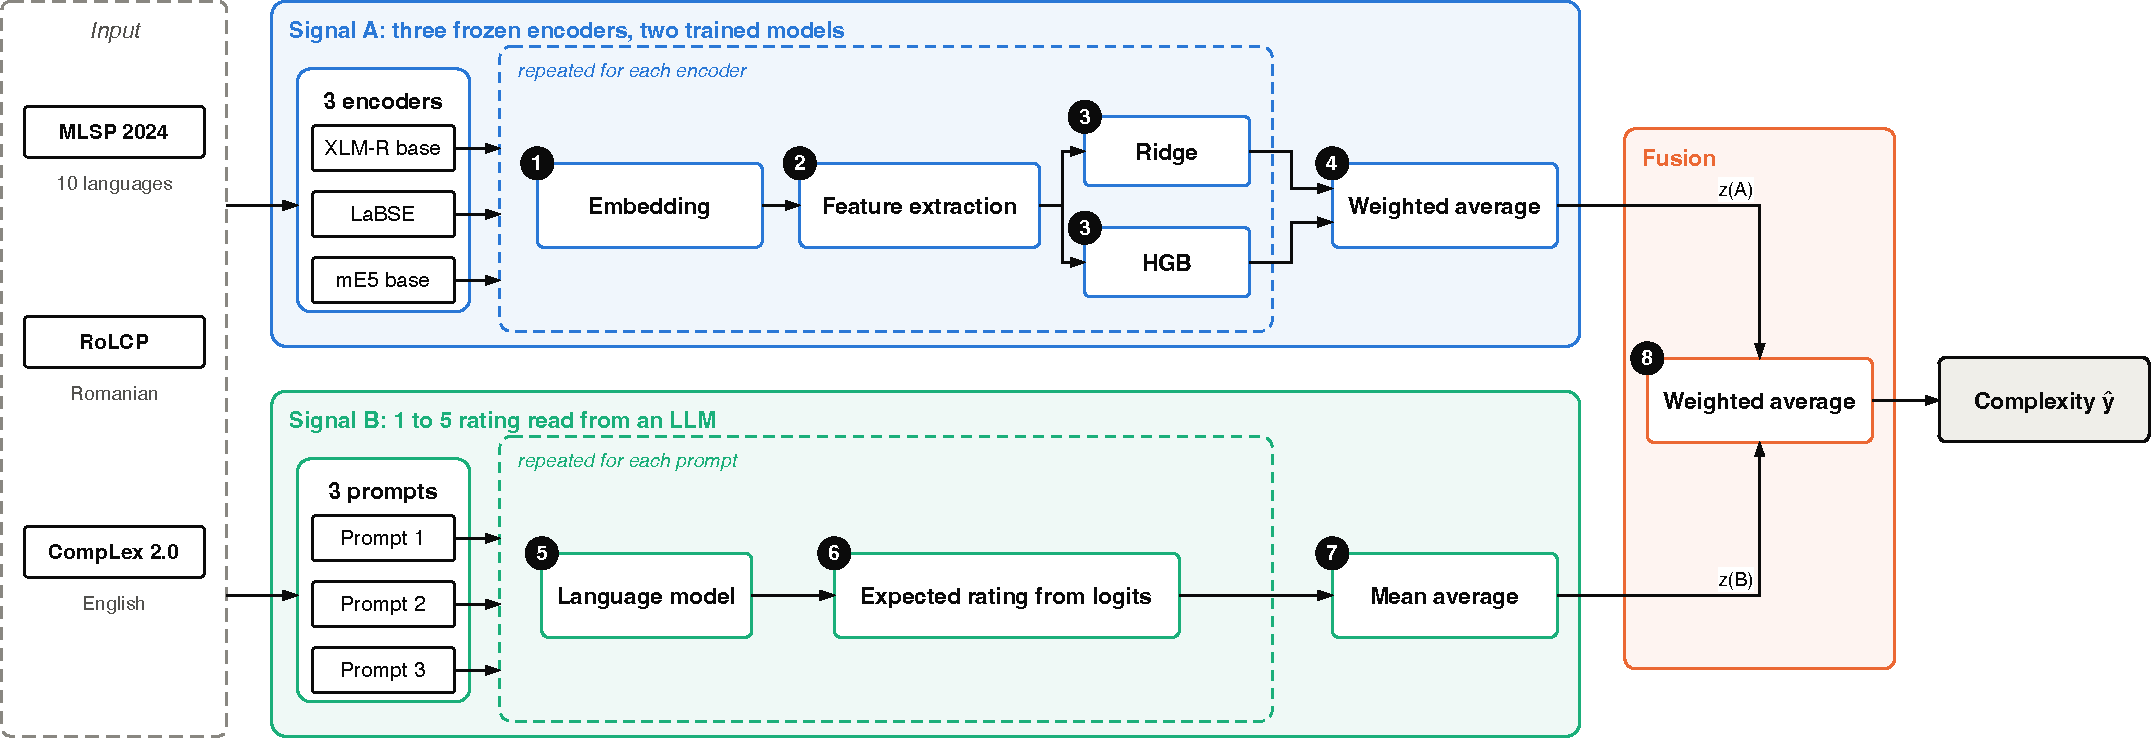
\includegraphics[width=\textwidth]{fig_pipeline_doc.pdf}
\caption{Overview of the pipeline for one held-out language. Signal~A (steps 1 to 4): each of
three frozen encoders embeds the target word in its context, the embedding is joined with lexical
features, and a ridge regression and a gradient-boosted tree predict complexity; the predictions
of the three encoders are then averaged. Signal~B (steps 5 to 7): a frozen language model rates the
target from 1 to 5 under three prompts, each rating is read from the probabilities of the digits,
and the three ratings are averaged. Step 8 fuses the two standardised signals.}
\label{fig:pipeline}
\end{figure*}

The method runs as two signals and a fusion (Figure~\ref{fig:pipeline}). Signal~A (steps 1 to 4)
is a regressor over three frozen multilingual encoders. Signal~B (steps 5 to 7) is a rating read
from the next-token probabilities of a frozen language model. Step 8 combines them. The ridge
regression and the gradient-boosted tree of step 3 are the only trained models. The encoders and
the language model keep their pretrained weights, and every other quantity is chosen on a grid.
Section~\ref{sec:protocol} states which labels each choice may use.

\subsection{Data}
\label{sec:data}

We evaluate on the test split of the MLSP 2024 lexical complexity data
\citep{shardlow-etal-2024-bea}: 5{,}624 target words in context % output/doc_counts.txt, "MLSP test rows: 5624"
in ten languages, Catalan, English, Filipino, French, German, Italian, Japanese, Portuguese, Sinhala
and Spanish. RoLCP \citep{anghel-etal-2025-rals} adds Romanian as an eleventh language, with
1{,}587 instances, % output/doc_counts.txt, randul ro
for 7{,}211 in total. % output/doc_counts.txt, "eval rows (11 langs): 7211"
Each instance is a context, a target word in it, and a complexity value between 0 and 1. % output/doc_counts.txt, coloanele y_min si y_max
No other MLSP 2024 split is used. Under the protocol of Section~\ref{sec:protocol} the test split
plays both roles: the labelled instances of the other languages are used for training and selection, and
those of the held-out language are scored.

The English CompLex 2.0 data \citep{shardlow-etal-2021-semeval} adds 8{,}423 labelled % output/doc_counts.txt, "CompLex 2.0 rows: 8423"
instances, from its single-word train, trial and test files. % release/data.py:33, COMPLEX_FILES
They serve only as training data for signal~A.

\subsection{Signal A}
\label{sec:signal-a}

Signal~A uses three multilingual encoders: XLM-R base \citep{conneau2020xlmr}, LaBSE
\citep{feng-etal-2022-language} and multilingual E5 base \citep{wang2024multilinguale5}. Steps 1
to 3 run separately for each encoder.

\paragraph{Step 1, embedding.} The context is cut to 500 characters on each side of the target % release/data.py:35, CHAR_WINDOW = 500
and passed through the encoder. % release/signal_a.py:48, .eval() si torch.no_grad(): ponderile nu se modifica
The target vector is the mean of the last four hidden layers, averaged over the subword tokens % release/signal_a.py:70
that overlap the target.

\paragraph{Step 2, feature extraction.} Each target vector is centred on the mean vector of its % release/signal_a.py:110-116, per_language
language, computed without labels. Six columns are appended. Fertility is the number of subword
units that the XLM-R tokeniser gives the target, centred in the same way. It replaces character % release/data.py:254-258, fertility
length, which is not comparable across writing systems \citep{rust-etal-2021-good}. Frequency is
the Zipf frequency from wordfreq \citep{speer-2022-wordfreq}, taken as the larger of the frequency
of the surface form and that of its lemma, with lemmas from stanza \citep{qi-etal-2020-stanza} run % release/data.py:231-251, lexical
on the full sentence. Filipino has no stanza lemmatiser, so only its surface forms are looked up. % release/data.py:29, STANZA_LANGS
Syllable count and capitalisation are defined only for Latin script. Two indicator columns mark a
language without a frequency list, which here is only Sinhala, and a language outside Latin script, % output/doc_counts.txt, "frequency available"
so that a missing value is never read as a small one.

\paragraph{Step 3, ridge and HGB.} A ridge regression ($\alpha = 300$, on standardised features
with median imputation) and a histogram gradient-boosted tree (HGB; depth 3, learning rate 0.05, % release/signal_a.py:97-100
400 iterations, L2 penalty 1.0) are fitted on the same rows, and their predictions are averaged.
The pair is fitted for two arms. The English arm, $p_{\mathrm{en}}$, is fitted once on CompLex and % release/signal_a.py:143
predicts every language. The multilingual arm, $p_{\mathrm{multi}}$, is fitted on CompLex plus the
labelled instances of every evaluation language except the held-out one, and is refitted for each % release/signal_a.py:145-151
held-out language. When English is held out, CompLex is removed from the multilingual arm and
$p_{\mathrm{en}}$ is set to $p_{\mathrm{multi}}$, so English is predicted without any English label.

\paragraph{Step 4, weighted average.} Within the held-out language, the predictions of each arm are % release/fuse.py:42-68, load_a
standardised for each encoder and averaged over the three encoders with equal weight. The two arms
are then mixed:
\begin{equation}
A = z\big(w_{\mathrm{src}}\, z(p_{\mathrm{en}}) + (1 - w_{\mathrm{src}})\, z(p_{\mathrm{multi}})\big),
\label{eq:arms}
\end{equation}
where $z$ standardises within the language and $w_{\mathrm{src}} \in \{0, 0.125, \dots, 1\}$ is % release/fuse.py:38, SRC_GRID
chosen in step 8.

\subsection{Signal B}
\label{sec:signal-b}

\paragraph{Step 5, language model.} Signal~B comes from Gemma~4 12B \citep{gemmateam-2026-gemma4}, % release/signal_b.py:38-39
instruction-tuned, in a 4-bit quantisation-aware-trained checkpoint run locally with MLX. No text
is generated, so each prompt costs one forward pass. The three % release/signal_b.py:117-135
prompts are in English and are zero-shot: each names the language, gives the sentence and the % release/signal_b.py:60-70, PROMPTS
target, and asks for a rating from 1 (very familiar) to 5 (very difficult), with no labelled
example. They differ in wording, and the third marks the target in the sentence with
\guillemotleft\,\guillemotright.

\paragraph{Step 6, expected rating from logits.} At the first answer position we take the
probability of the tokens \texttt{1} to \texttt{5} and renormalise it over the five digits. The % release/signal_b.py:125-135, digit_probs
distribution is sharpened or flattened with a temperature $T$, raising each probability to $1/T$ % release/fuse.py:79-83, temper
and renormalising, and contiguous digits may be merged into blocks, each valued at the mean of its
digits. For one prompt the rating is % release/fuse.py:86-89, b_of
\begin{equation}
B = \frac{1}{4}\Big(\sum_{b} P_b\, v_b - 1\Big),
\label{eq:rating}
\end{equation}
where $P_b$ is the tempered probability of block $b$ and $v_b$ its value, so $B$ lies between 0
and 1.

\paragraph{Step 7, mean average.} $B$ is the mean of the three prompt ratings, with equal weight. % release/fuse.py:89

The language model never sees a label. Three quantities are
selected on a grid by mean correlation over the other languages. $T$ is chosen first, among 16 % release/fuse.py:32, T_GRID
values from 0.5 to 64. The partition is chosen next, among the 15 ways of splitting the five digits % release/fuse.py:34-35, PARTITIONS
into two to five contiguous blocks. The language model is chosen among three candidates: % release/fuse.py:165-171, pick_model
Gemma~4 and two smaller models, Qwen3 8B \citep{yang-etal-2025-qwen3} at 4 bits and Qwen3.5 9B at % release/README.md, sectiunea Models
8 bits. For the two Qwen models only the mean rating of two prompts at $T = 1$ was stored, over the
ten MLSP languages. Gemma~4 is selected for every language. % output/doc_fuse_ro11.txt, coloana model

\subsection{Fusion}
\label{sec:fusion}

\paragraph{Step 8, weighted average.} Both signals are standardised within the language and
combined:
\begin{equation}
\hat{y} = w\, z(A) + (1 - w)\, z(B),
\label{eq:fusion}
\end{equation}
with $w \in \{0, 0.05, \dots, 1\}$. The pair $(w_{\mathrm{src}}, w)$ is chosen on the other % release/fuse.py:37, W_GRID
languages, which we call the fitting languages, by a nested criterion. A candidate % release/fuse.py:191-205, fit
$w_{\mathrm{src}}$ is scored by its mean correlation over the fitting languages, where the $w$
applied to each fitting language is fitted on the remaining ones. The best $w_{\mathrm{src}}$ is
kept, and $w$ is then fitted on all fitting languages. The signals of a fitting language are its
own held-out predictions, built in the same way.

\subsection{Evaluation Protocol}
\label{sec:protocol}

All results use the same protocol, leave-one-language-out (LOLO). Each language is held out in
turn, and everything applied to it is fitted or chosen on the other languages: the multilingual
arm of signal~A, $w_{\mathrm{src}}$, $T$, the partition, the language model and $w$. The held-out
language contributes only its unlabelled inputs, to centre the embeddings and to standardise the
predictions. Its labels do not enter its own predictions directly. They can reach them only at
second order, through the held-out predictions of the fitting languages, which we discuss among
the limitations.

We score each language by the Pearson correlation between predictions and gold values on its
instances, and report the unweighted mean over languages. Confidence intervals resample contexts
rather than instances, because several targets often share a sentence. We draw 2{,}000 bootstrap % release/fuse.py:214, --boot 2000
resamples of contexts in each language and report 95\% percentile intervals. The interval of the % release/fuse.py:252-256
mean averages the $k$-th resample over languages.

% =====================================================================
\section{Experimental Results}
\label{sec:results}
% PAS 3.

\subsection{Per-Language Results}
\label{sec:per-language}
% Tabel: cele 11 limbi, cu n, r pentru A, B si fuziune si CI de 95%, plus
% media. Sursa: output/doc_fuse_ro11.txt.

\subsection{Ablations}
\label{sec:ablations}
% Tabel cu ce scoate fuse.py: 10 limbi MLSP (rulare separata, romana scoasa
% si din antrenare), un singur encoder, patru encodere, un singur LLM.
% Qwen nu are romana, deci ablatia de LLM se face pe 10 limbi.

\subsection{Comparison with Published Results}
\label{sec:published}
% Tabel pe cele 10 limbi MLSP: baseline de frecventa, Archaeology, TMU-HIT
% zero-shot si per-language best, G-Eval, G-Scale, noi (rularea pe 10).
% Media pe limbi, nu pooled. Se spune care rezultate folosesc etichete din
% limba tinta.

\subsection{Feature Attribution}
\label{sec:shap}
% Figura SHAP pe semnalul A (figures/fig_shap_signal_a.pdf) si cifrele din
% output/shap_signal_a_adopted_importance.csv.

\subsection{Representation Geometry}
\label{sec:tsne}
% Figura t-SNE inainte si dupa centrare (figures/fig_tsne_encoders.png) si
% ponderea vecinilor din aceeasi limba.

% =====================================================================
\section{What Did Not Work}
\label{sec:negative}
% PAS 4. Lista de experimente ceruta de curs, pe buline: fiecare axa
% inchisa intr-o propozitie, cu cifra ei. Lista se aproba intai in chat.

% =====================================================================
\section{Conclusions and Future Work}
\label{sec:conclusions}
% PAS 6. Ca in glioma, paragrafe cu titlu bold. Limitations e
% \section*{Limitations} din sablon, mai jos.

\paragraph{Conclusions.}
% Ce am facut si cifrele principale, fara idei noi.

\paragraph{Future Work.}
% Pe buline, ca in glioma.

% =====================================================================
\section*{Implementation}
% PAS 6. Ca in glioma: link-ul repo-ului anonim, uneltele, timpii de rulare
% din README si masinile pe care s-a rulat.

% =====================================================================
\section*{Limitations}
% PAS 6. Al treilea prompt ales pe test; configuratiile masurate pe test si
% alegerea intre ele; dependentele de ordinul doi din LOLO; Known
% limitations din README.

\section*{Acknowledgments}
% Din sablon, cu cele doua declaratii din paperul de glioma.
% Seturile de date: release/README.md, sectiunea Data, si release/data.py.

\begin{itemize}
\item Conflicts of Interest: The authors have no conflicts of interest or competing interests to
declare in the context of this paper.
\item Data Sharing: All experiments use publicly released datasets: MLSP 2024
\citep{shardlow-etal-2024-bea}, CompLex 2.0 \citep{shardlow-etal-2021-semeval} and RoLCP
\citep{anghel-etal-2025-rals}.
\end{itemize}

% Schela pentru pasul 1: tipareste toata bibliografia de pornire ca sa se
% poata verifica in PDF. SE SCOATE cand textul are citari (cel tarziu la pasul 8).
\nocite{*}

% Bibliography entries for the entire Anthology, followed by custom entries
%\bibliography{custom,anthology-overleaf-1,anthology-overleaf-2}

% Custom bibliography entries only
\bibliography{custom}

\appendix

% Anexa din sablon (\section{Example Appendix} \label{sec:appendix}).
% Continutul nu e decis; prompturile lui B au fost oferite ca anexa.
% Fara \section aici, \appendix nu tipareste nimic.

\end{document}
